\documentclass[11pt,letterpaper]{article}
\usepackage[T1]{fontenc}
\usepackage[utf8]{inputenc}
\usepackage{lmodern,microtype}
\usepackage[margin=1in,headheight=15pt]{geometry}
\usepackage{amsmath,amssymb,amsthm,mathtools}
\usepackage{booktabs,tabularx,longtable,array,enumitem}
\usepackage{xcolor,listings,tikz,needspace,fancyhdr,titlesec,etoolbox}
\usetikzlibrary{arrows.meta,positioning}
\usepackage{xurl}
\usepackage[colorlinks=true,linkcolor=blue!45!black,citecolor=blue!45!black,urlcolor=blue!45!black]{hyperref}
\usepackage{bookmark}
\definecolor{ink}{HTML}{19354A}
\definecolor{accent}{HTML}{217A83}
\definecolor{pale}{HTML}{F0F5F7}
\titleformat{\section}{\Large\sffamily\bfseries\color{ink}}{\thesection}{.65em}{}
\titleformat{\subsection}{\large\sffamily\bfseries\color{ink}}{\thesubsection}{.65em}{}
\pretocmd{\section}{\Needspace{6\baselineskip}}{}{}
\pretocmd{\subsection}{\Needspace{6\baselineskip}}{}{}
\BeforeBeginEnvironment{lstlisting}{\par\noindent\begin{minipage}{\linewidth}}
\AfterEndEnvironment{lstlisting}{\end{minipage}\par}
\setlength{\parskip}{.38em}
\setlength{\parindent}{0pt}
\setlength{\emergencystretch}{2em}
\setcounter{tocdepth}{1}
\setlist{nosep,leftmargin=*}
\renewcommand{\arraystretch}{1.16}
\newcolumntype{Y}{>{\raggedright\arraybackslash}X}
\newcolumntype{P}[1]{>{\raggedright\arraybackslash}p{#1}}
\newcommand{\code}[1]{\nolinkurl{#1}}
\newcommand{\R}{\mathbb R}
\newcommand{\N}{\mathbb N}
\newcommand{\Z}{\mathbb Z}
\newcommand{\Q}{\mathbb Q}
\newcommand{\decision}[1]{\par\smallskip\textbf{Recommendation.} #1\par\smallskip}
\newtheorem{proposition}{Proposition}
\lstset{basicstyle=\small\ttfamily,columns=fullflexible,keepspaces=true,
breaklines=true,frame=single,rulecolor=\color{accent!35},backgroundcolor=\color{pale},
aboveskip=.7em,belowskip=.7em,showstringspaces=false}
\pagestyle{fancy}
\fancyhf{}
\fancyhead[L]{\small\sffamily Mathematical objects, certified computation}
\fancyhead[R]{\small\sffamily Round 2 synthesis}
\fancyfoot[C]{\thepage}
\hypersetup{pdftitle={Mathematical Objects, Certified Computation: A Unified Evaluation of Nine Proof-Language Proposals},pdfauthor={Codex, prepared for Vladimir Reshetnikov},pdfsubject={Self-contained synthesis of Accord, Cadence, Concord, Facet, Locus, Meridian, Noema, Prism, and Vantage}}
\begin{document}
\hypersetup{pageanchor=false}
\begin{titlepage}
\color{ink}
{\sffamily\large LANGUAGE DESIGN / ROUND 2\par}
\vspace{1.15in}
{\sffamily\bfseries\fontsize{31}{36}\selectfont Mathematical Objects,\\Certified Computation\par}
\vspace{.35in}
{\sffamily\Large A unified evaluation of nine proposals\\for a more natural mathematical proof language\par}
\vspace{.5in}
{\large Accord, Cadence, Concord, Facet, Locus,\\Meridian, Noema, Prism, and Vantage\par}
\vfill
\rule{\textwidth}{1pt}
Prepared for Vladimir Reshetnikov\par
Codex, with parallel source reviews and independent mathematical checks\par
6 September 2026 (UTC)\par
\vspace{.3in}
\textbf{Reading contract.} This report is self-contained. It explains the inherited
design ideas before evaluating their extensions. The cited proposals and earlier
syntheses provide provenance and further detail; none is a prerequisite.
\end{titlepage}
\hypersetup{pageanchor=true}

\section*{Executive assessment}
\addcontentsline{toc}{section}{Executive assessment}
The nine proposals converge on a useful architectural direction: let mathematicians
work with ordinary mathematical objects, and let computations return checked,
explicitly limited information about those objects. A polynomial presentation, a
finite power-series jet, an interval enclosure, and a symbolic solution set should
not all masquerade as equality. Each has its own mathematical contract. This is
the strongest advance in the second round.

The practical opportunity is broader than prettier Lean syntax. A mathematician
should be able to request a coefficient, choose an induction argument, change
representation, or ask for a solution without manually supplying every transport
lemma and intermediate witness. Yet the system must preserve the intended
statement, expose conditions that affect its meaning, and retain evidence that
can be checked after exploratory automation has disappeared. Lean can remain the
initial proof backend; a new kernel is neither required nor justified by these
reports.

There is substantial agreement on eight broad commitments, with explicit source
support in all nine reports: relation-specific computational results; fixed
semantic objects and certified presentations or observations; scoped guards;
justified execution and reification; theorem-based interfaces separate from
search policy; exact-target proof providers; retained replay evidence; and a fair
comparison with equally equipped Lean. This is agreement among proposals that
share earlier syntheses and examples, not nine independent empirical validations.
The substantive differences concern which computation to implement first, how
much representation change to automate, and how much evidence the author must
see during ordinary work.

The best contributions combine naturally. Facet and Vantage sharpen the meaning
of a representation. Noema and Cadence make conditional results and composition
precise. Locus supplies a particularly good residual-to-jet theorem. Meridian and
Prism develop symbolic calculus with an arbitrary derivative index. Accord
emphasizes executable certificates and reusable theorem interfaces. Concord
keeps finite computation attached to an arbitrary formal solution. None provides
an implemented end-to-end language or a Lean-verified CAS subsystem. All nine
Python companions ran successfully in this review, but their finite checks use
different units and establish much less than those implementation goals.

I recommend a shared typed request-and-evidence protocol, first exercised by
guarded polynomial/rational computation and one formal-series residual problem.
Expose the same theorem packages and computation services through ordinary Lean
and a small mathematical frontend. Measure whether the frontend improves
semantic understanding and maintenance after including infrastructure cost.
Keep local differentiation, parameter-degenerate solving, and hostile
certificate mutations as discriminating tests. A successful theorem library and
linter is a legitimate outcome if additional syntax brings no measurable gain.

The additional synthesis \emph{Nine Workbenches} strengthens the case for an
early Lean prototype with toolchain probes and a consolidated mutation catalogue.
This revision incorporates those contributions, qualifies its performance and
novelty claims, and adds explicit tests of its proposed implication rules. The
remaining work is proving and integrating a checker, not merely timing its Boolean result.

\clearpage
\tableofcontents
\clearpage

\section{Scope, sources, and the meaning of evidence}\label{sec:evidence}
This report synthesizes the nine packages in \code{docs/round-2/ideas}, as imported
at Git commit \code{f333ff6cefc8b1f5c9aae79613d10ef95a7ba928}. The current branch
was fast-forwarded to that fetched \texttt{main} revision before review. All nine
TeX reports, their mathematical examples, companion programs, recorded results,
and provenance notes were reviewed. Three parallel reading lanes each covered
three complete reports; the synthesis also directly inspected the central
definitions and mathematical cases. Appendix~\ref{app:crosswalk} provides a
source crosswalk, and the adjacent JSON registers provide exact file hashes and
one-based TeX line locators.

Two first-round syntheses are part of the intellectual provenance: the earlier
Codex report and the Claude report, including its Leant discussion and subsequent
questions \cite{round1,claude}. Their relevant concepts are explained in
Section~\ref{sec:baseline}; their questions are restated and assessed in
Appendix~\ref{app:oldquestions}. The new report does not require their vocabulary
or argument to be remembered.

This revision also reviews Claude's second-round synthesis, \emph{Nine
Workbenches}, its tables, generator, and Lean experiment sources and logs
\cite{secondary}. It was imported by a fast-forward merge of fetched
\texttt{main} at \code{84af03f49f89a31b47ff3416ccdbc9180fd6b438}.
It is treated as a secondary analysis, not a tenth independent proposal. A
separate register under \code{evidence/secondary-review} pins its 17 files;
the original nine-report source register and crosswalk retain their original scope.

\subsection{What was reproduced}
The original input packages were left unchanged. Their Python companions were
run with bytecode generation disabled and output redirected into this synthesis's
evidence directories. All nine completed successfully under Python 3.14.4.
Comparisons with shipped results are recorded per package; interpreter metadata
can differ without changing the arithmetic result.

\begin{center}\small
\begin{tabularx}{\textwidth}{@{}P{.9in}P{1.5in}Y@{}}
\toprule
Report & Fresh companion result & What the count means\\
\midrule
Accord & 25 tests & Unit-test methods covering several certificate families.\\
Cadence & 267 checks & Reported finite arithmetic and negative examples.\\
Concord & 459 checks & Includes 441 binomial instances and seven negative cases.\\
Facet & 1,100 checks & Finite checks across its mathematical families.\\
Locus & 24 tests & Includes 702 binomial instances and jets through order 24.\\
Meridian & 27 tests & Reported exact-arithmetic test cases.\\
Noema & 25 tests & Includes 182 binomial instances inside one test method.\\
Prism & 2,475 checks & Reported finite instances; certificate output reproduced.\\
Vantage & 3,013 checks & Reported instances in ten groups.\\
\bottomrule
\end{tabularx}
\end{center}

These figures must not be added into a proof count or used to rank languages.
A thousand evaluations of one identity and a test of one malformed certificate
answer different questions. Several producer and checker prototypes share
arithmetic code. Reproduction establishes that the supplied executable examples
behave as reported in this environment; it does not establish a sound compiler,
a verified checker, a universal theorem, or improved author productivity.

\subsection{Four distinct kinds of support}
Throughout the report, \emph{proposed} means an interface or policy is described;
\emph{mathematically justified} means an argument with stated hypotheses is
given; \emph{executed} means a particular program was run on specified inputs;
and \emph{kernel checked} means an actual proof was accepted by the stated Lean
environment. These descriptions are not interchangeable. The focused Lean
experiments in the accompanying evidence establish only their
listed declarations, not the larger language design.

Leant and ProveIt motivate important examples. This synthesis uses the reports'
source-attributed observations and the prior review as historical evidence; it
does not present those observations as a fresh audit of every file in today's
external checkouts. Any new Lean experiment is isolated in the synthesis
directory and uses existing dependencies read-only. No external repository is
modified or rebuilt for this report.

Some input READMEs refer to checksum artifacts absent from the imported tree.
The source register therefore records independently computed hashes of the files
actually present. Missing packaging artifacts are not silently reconstructed,
and source-manifest assertions are not elevated into fresh validation receipts.

\section{The problem and the inherited design, explained afresh}\label{sec:baseline}
Lean's value is that a compact trusted checker can validate explicit proof terms
in a precise foundational language. Its elaborator reconstructs omitted
information, resolves notation and instances, and translates tactics into terms.
A mathematician, however, usually organizes an argument by objects, useful
representations, intermediate claims, and reasons. Much formalization work lies
between those two levels: finding the correct theorem, aligning its hypotheses,
transporting statements between equivalent representations, and exposing facts
that paper mathematics leaves locally understood.

These are several different problems. A short proof can conceal a changed
statement. A long proof can be a reusable general theorem rather than accidental
verbosity. A missing automation rule may require a library improvement, while
an unclear scope or hidden domain change may require a language or interface
improvement. A sound evaluation must identify which cost it actually removes.

\subsection{A mathematical step with a checked reason}
Consider an author writing, ``Reindex the sum by \(k=j+i\), then use the binomial
theorem.'' A useful interface should retain both claims and their reasons. It
can elaborate the first step using a theorem about a bijection of finite index
sets, with explicit obligations for bounds, injectivity, surjectivity, and
summand equality. Routine arithmetic can solve those obligations. The author's
reason then constrains the accepted derivation: an unrelated global automation
success should not pretend to validate the advertised reindexing.

The economical implementation is often an \emph{annotated theorem interface}.
An ordinary Lean theorem supplies the logical contract. Additional metadata
names semantic roles such as source set, target set, map, and transport proof.
Separate policy chooses search order, display defaults, and routine solvers.
This division lets the theorem remain useful in ordinary Lean, and prevents
search priorities from becoming mathematical axioms. Stable wrapper declarations
and role identifiers can insulate the interface from upstream binder renaming,
but compatibility still needs checking after refactoring.

A larger \emph{method ledger} records the tree of accepted steps: requested
claim, selected method, generated obligations, their proofs, and dependencies.
It can support readable explanations and repair. It is not automatically needed
for every first prototype. Start with a small theorem interface and retain the
data required by a specific user-facing function; do not build an entire method
language before demonstrating its value.

\subsection{Statements, routine work, and definitions}
A \emph{statement seal} is a readable account of what the system has actually
elaborated: quantified variables, their types, active hypotheses, ambient
algebraic structure, domain and branch conventions, and significant implicit
choices. It is useful because a kernel proves the elaborated proposition,
whereas the author intended a proposition expressed through notation and
context. Those can diverge without any kernel error. A seal is an inspectable
interface and linting boundary, not a theorem that the author meant the result.

\emph{Routine profiles} specify which obligations automation may discharge
without distracting the author. Examples include linear arithmetic, a fixed
normalization procedure, or a named simplification set. They need explicit
resource bounds, reproducible package identities, and a policy for changed
outcomes. ``Routine'' is a project convention that must be measured on realistic
work; it is not synonymous with mathematically trivial or computationally cheap.

Definition design deserves the same attention as proof steps. A definition
package may supply an ordinary semantic definition, characterizing equations,
existence and uniqueness theorems, executable presentations, observations, and
transport laws. Introducing an arbitrary object satisfying a specification is
different from constructing one algorithmically, and both differ from selecting
one by noncomputable choice. A frontend may make these activities concise, but
must preserve the distinction and generate genuine obligations rather than
assuming the desired laws.

\subsection{Suggestions and retained evidence}
An automatic provider proposes a term or tactic for an exact goal in an exact
context. Acceptance requires validation at that target. The displayed tactic
must itself be replayed after insertion: a search tactic may work while the
shorter text it prints fails, leaves goals, or affects surrounding syntax.
Successful elaboration with an admitted hole does not establish a complete
proof. Search failure, resource exhaustion, and a mathematical refutation are
different outcomes.

During exploration the system may search widely. Publication should retain the
accepted terms or certificates, their source interpretation, and the environment
needed for deterministic checking. A script that rediscovers a proof, a saved
proof term, and a compiled artifact serve different replay purposes. Upgrading a
library is a new checking event with a migration receipt; a previously valid
artifact is not evidence that migration succeeded.

These principles explain the second round's starting point. Its important new
question is how to extend them from proof steps to computation over mathematical
objects without losing domains, precision, or the author's chosen object.

\section{Where the nine reports converge}\label{sec:convergence}
Appendix~\ref{app:crosswalk} and \code{convergence.json} document eight broad
commitments, each explicitly proposed by all nine reports. The feature
definitions are deliberately precise about their breadth. ``Separate verified
algorithms from execution,'' for example, is a design commitment, not a claim
that every report gives equally detailed executable semantics.

\begin{center}\small
\begin{tabularx}{\textwidth}{@{}P{.3in}P{1.55in}Y@{}}
\toprule
 & Shared commitment & Practical implication\\
\midrule
R & Relation-specific result & Record equality, domain equality, jet agreement,
enclosure, witness correctness, or coverage as different specifications.\\
O & Fixed semantic object & Computable presentations and observations refer to
the original object; a convenient replacement needs a theorem.\\
G & Scoped guards & Carry conditions through dependent composition; do not
silently narrow the requested domain or add a hypothesis.\\
V & Verified execution boundary & Prove the checker or algorithm, justify its
actual execution, and connect reified syntax to the original expression.\\
D & Theorem and definition packages & Keep logical contracts usable in Lean;
version search and presentation policy separately.\\
L & Exact-target providers & Replay the actual edit, inspect completion, and
avoid promoting abstract search failure to a negation.\\
P & Retained publication evidence & Check accepted assertions from retained
evidence in a pinned environment without renewed discovery.\\
E & Fair empirical evaluation & Equip Lean with the same services; include
negative neighbors, maintenance cost, and an explicit stopping decision.\\
\bottomrule
\end{tabularx}
\end{center}

This convergence supports a common prototype architecture. It does not settle
the interface. An exact object plus a relation is a strong semantic foundation,
but it can support a notebook, a textual proof language, a structured document
editor, or Lean commands. Likewise, retaining proof evidence does not determine
whether authors usually see a one-line result or an expanded obligation tree.

The agreement is also correlated. The reports share the same two earlier
syntheses and many ProveIt examples. Several deliberately preserve the same
adversarial boundaries. That is useful refinement, but it makes a nine-way vote
a poor measure of independent confidence. A genuinely new round should include
held-out mathematical work and readers who did not help design the notation.

\subsection{Distinctive contributions worth preserving}
\textbf{Accord} is strongest as a disciplined certificate architecture. It
separates mathematical answer kinds from validation states, gives reification a
dedicated role, and connects theorem interfaces to publication checks. Its
radical-denesting development makes branch selection part of a general
contract rather than a successful numerical identity. Its initial slice,
finite reindexing plus polynomial certificates, is conservative and useful,
although by itself it could be delivered mostly as a Lean library
\cite[\S\S5--8,12--17]{accord}.

\textbf{Cadence} emphasizes the composition of guarantees: finite precision,
conditional simplification, and complete solution sets. The all-parameter
equation \(ax=b\) is a particularly good first example because specialization
can change both existence and the number of solutions. Cadence asks whether
actual execution is justified, not merely whether the source algorithm has a
correctness theorem. Its broad agenda makes adherence to its small first slice
important; numerical evaluation gates should follow a pilot and precede the main comparison
\cite[\S\S4--7,9--10,15--18]{cadence}.

\textbf{Concord} makes finite residual certificates central. It shows how a
polynomial can establish a finite observation about an arbitrary fixed-point
series without changing that series into a canonical implementation. Its
separation of nonderivability from negation is essential to provider design.
The first slice is mathematically distinctive, but the general bridge from
formal residuals to observations still needs Lean implementation
\cite[\S\S4--7,10,13,15,17]{concord}.

\textbf{Facet} usefully observes that an exact decoding map does not require a
general encoder. A noncomputable semantic object may still have a certified
presentation supplied by a producer. Observation handles distinguish a finite
answer from a replacement object, and its Abel example maintains that distinction
under general algebraic assumptions. The main implementation risk is allowing
the generality of the presentation framework to precede a demonstrated workflow
\cite[\S\S4--6,9,11--15]{facet}.

\textbf{Locus} supplies the clearest small theorem that links symbolic computation
to an infinite semantic object: a sufficiently small residual and a unit
derivative identify a finite jet of an existing formal root. This gives a
concrete correctness boundary for truncation and Newton refinement. Its dyadic
germ is a promising first vertical slice. Existence of the original root and
execution of the truncation algorithm remain separate proof obligations
\cite[\S\S4--8,12--14]{locus}.

\textbf{Meridian} is especially careful about partial-function domains,
substitution guards, and solution predicates. Its Lambert derivative family
connects a symbolic index, polynomial arithmetic, analytic differentiation, and
local hypotheses. It also warns that an injective map such as \(\Z\to\Q\)
does not reflect every richer algebraic claim. This is an excellent stress test
for transport metadata. Meridian itself chooses partial-rational computation
and domain-preserving solving first, with Lambert calculus as a second slice
\cite[\S\S4--9,12--16]{meridian}.

\textbf{Noema} provides the most compact account of relation-bearing requests
and sufficient guards. It does not promise weakest guards or a universal
ordering of result types. Its executable cancellation example binds evidence to
the request, revision, scope, and required denominators. Stable semantic role
identifiers give a practical method-interface design. The prototype is a useful
boundary model, not an implementation of dependent contexts or proof checking
\cite[\S\S4--8,10--12]{noema}.

\textbf{Prism} combines a strong symbolic-calculus case with demand-driven
precision. It also makes an ergonomic point worth retaining: an author may
delegate witness construction by specification; safety does not require asking
permission for every discovered formula. The accepted witness still needs the
same contract and provenance. The implementation challenge is to preserve these
precise semantics without making every ordinary request resemble a protocol
configuration form \cite[\S\S5--7,9--11,13--18]{prism}.

\textbf{Vantage} offers the sharpest taxonomy: exact presentations, restricted
observations, and directed abstractions are different tools. Its normalized EGF
interface, developed through Touchard, Bell, and Spivey identities, makes
definition and observation design concrete. It also gives a decisive logical
example of why failed intuitionistic search is not negation. Some illustrative
contracts still need edge hypotheses, including ordered bounds for its
telescoping example; this reinforces the value of negative neighbors
\cite[\S\S3,5,9--15]{vantage}.

\subsection{What a finer tally adds, and what it cannot count}
\emph{Nine Workbenches} supplies a finer matrix of 58 commitments, coding 40 as
unanimous and 44 as explicit in at least seven reports \cite[\S4]{secondary}.
Those totals reproduce from its supplied data. They complement this report's
eight broader commitments: a report can explicitly support the broad execution
boundary while discussing a particular execution mechanism only partially.
The two matrices therefore answer different questions and should not be
combined into one score.

The finer matrix is manually authored editorial coding. Its generator serializes
the assigned marks; it does not discover or validate them by reading the reports.
Similarly, the reported 30 unanimous ``new'' rows are the unanimous rows outside
the group named ``Inherited foundation.'' That grouping is not a demonstrated
novelty boundary. Exact displayed-edit replay, original-target negative evidence,
transactional validation, and preservation versus reflection already appear in
the earlier syntheses. The
valuable addition is finer comparison and disagreement detection, not a count
of independently discovered ideas. Nor does agreement on high-level answers
settle the operational choices and empirical questions restated in
Appendix~\ref{app:oldquestions}.

\subsection{What the convergence does not establish}
No report demonstrates that a new input language beats a good theorem library
with an equally capable computation service. None settles the cost of checking
large certificates or reifying realistic expressions. None measures whether
authors notice a weakened result or correctly interpret a compact display. The
reports supply enough agreement to stop inventing nine separate architectures;
they do not supply enough evidence to freeze the surface language.

\section{A common semantic model}\label{sec:model}
The common design can be expressed without committing to a new grammar. A
request identifies a mathematical context \(\Gamma\), an object \(x\), an
operation or observation, and a required specification. A producer returns data
\(y\), proposed supporting evidence, and any remaining conditions. Acceptance
requires a proof of the requested relation at the original target.

For a conditional transformation, the essential judgment is
\[
  \Gamma\vdash p : G \longrightarrow \mathcal R(x,y).
\]
It becomes an unconditional fact in \(\Gamma\) only when the guard \(G\) is
proved there. The guard may depend on the input, the output, and prior choices.
The relation \(\mathcal R\) is part of the mathematical specification, not a
display tag attached after a computation has finished.

Sometimes the result itself depends on guard evidence. The dependent type
\(\prod_{h:G}\sum_y\mathcal R(x,y)\) allows such a witness-dependent result;
it is not the same interface as \(\sum_y\prod_{h:G}\mathcal R(x,y)\), which
selects one result before receiving the guard proof. Facet makes this scope
distinction explicit \cite[\S5.2]{facet}. A general request protocol must
preserve it even if the first prototype supports only simpler fixed-output cases.

\subsection{Three representation relationships}
An \emph{exact presentation} consists of data \(r\), a meaning map
\(\lbrack\!\lbrack r\rbrack\!\rbrack\), any validity condition, and a proof that its meaning
is \(x\). There need not be a computable function that encodes every semantic
object. For example, a polynomial representation of a function may be supplied
and proved correct even when the function was introduced abstractly.

A \emph{restricted observation} supplies only some requested information:
\(r\) agrees with \(x\) on a domain, computes its first \(N\) coefficients, or
encloses a value. It is generally not legitimate to replace \(x\) everywhere by
\(r\). Two observations need only be coherent where their guarantees overlap.
Different valid enclosures can have different widths; neither needs to equal
the other as an interval.

A \emph{directed abstraction} maps a problem into a simpler language for a
particular inference. Its correctness theorem determines which conclusions
transport in which direction. A sound prover for an abstraction may establish
original claims if each accepted proof reconstructs correctly; its failure
does not automatically establish original impossibility. Exact decoding,
observational adequacy, and abstract-search adequacy are separate contracts.

\subsection{Kinds of computational answer}
\begin{center}\small
\begin{tabularx}{\textwidth}{@{}P{1.15in}Y Y@{}}
\toprule
Answer & Required guarantee & A tempting invalid promotion\\
\midrule
Exact transformation & \(x=y\) in the specified structure & Equality after a
noninjective map becomes equality before it.\\
Equality on a domain & \(\forall u\in D,\ f(u)=g(u)\) & Equality on \(D\) becomes
global equality, or \(D\) silently shrinks.\\
Finite jet & Coefficients agree for every \(k<N\) & Finite agreement becomes a
formal identity or analytic error estimate.\\
Enclosure & \(\ell\le x\le u\), with stated endpoint convention & A floating
midpoint becomes an exact value.\\
Witness & \(P(y)\) & One root becomes every root.\\
Complete solutions & \(\forall y,\ P(y)\leftrightarrow S(y)\) & Generic
parameter assumptions disappear under specialization.\\
Factorization & Product identity plus requested factor properties & Product
equality becomes irreducibility or uniqueness.\\
\bottomrule
\end{tabularx}
\end{center}

Exact equality of partial functions additionally requires identical definedness
domains and equal values there; equality on a shared subset is weaker.
There is no useful universal ``confidence level'' ordering these answers. A
complete solution predicate and an accurate enclosure can be incomparable.
Even where guarantees admit weakening, the weakening needs an actual theorem:
precision \(N\) implies precision \(M\le N\), while an interval bound implies
a looser interval only after endpoint inequalities are established.

\subsection{Implication rules need all their hypotheses}\label{sec:bridges}
The secondary synthesis usefully proposes an explicit catalogue of bridges
between computational guarantees \cite[\S9.1]{secondary}. Its table should
be implemented as a registry of proved implications between precise predicates,
not as a universal ordering or a closed inventory of every possible result.
Three entries need repair before becoming contracts.

\textbf{A complete solution set requires soundness and coverage.} For a set
\(S\), the required statement is \(\forall x,\ P(x)\leftrightarrow x\in S\).
One needs both \(\forall x\in S,\ P(x)\) and
\(\forall x,\ P(x)\to x\in S\). A single witness \(P(w)\) plus coverage does
not establish soundness. For example, \(P(x)\) meaning \(x=0\),
\(w=0\), and \(S=\{0,1\}\subseteq\Z\) satisfy the witness and coverage
claims, but \(S\) contains an extraneous solution.

\textbf{Openness does not strengthen a pointwise identity.} To obtain equality
near \(x\), an open set \(U\) containing \(x\) helps only when the functions
agree \emph{throughout} \(U\). The real line is open, yet \(f(t)=t\) and
\(g(t)=0\) agree at zero without agreeing near zero. The missing premise is
the identity on the neighborhood, not openness by itself.

\textbf{Some enclosures do establish equality.} From
\(\ell\le x\le u\) and \(\ell=u\), antisymmetry gives \(x=\ell\).
Thus the secondary table's ``never'' is too strong. A nondegenerate enclosure
generally gives only bounds; equality can follow from collapsed bounds or an
appropriate limiting theorem. Likewise, an interval containing zero does not
by itself establish a strict sign, although its endpoints can still establish
non-strict bounds.

These repairs suggest a test for the bridge registry itself: deliberately omit
one premise, then demand that the invalid promotion fail even when the producer's
underlying computation is correct. Checking a certificate and checking that its
guarantee answers the user's question are different obligations.

\subsection{Composition is dependent and directional}
Suppose a first stage yields \(y\) with \(G_1\to\mathcal R_1(x,y)\), and a
second stage yields \(z\) with \(G_2(y)\to\mathcal R_2(y,z)\). A composition
theorem may establish \(\mathcal R(x,z)\) under both guards. The intermediate
\(y\) must be bound before \(G_2(y)\) is formed. An implementation cannot
flatten these conditions into unrelated strings or move them across a witness
scope without justification.

Equality on domains composes on their intersection. That does not authorize
answering a request for equality on \(D\) with equality on a smaller set: the
system must prove that the required \(D\) lies in the available domains, branch
the task, or report a conditional result. Numerical error composition needs
triangle inequalities or stability bounds. Differentiation requires a local
equality theorem rather than arbitrary pointwise replacement.

Guards should initially be \emph{sufficient}, not advertised as weakest. A
method may require a nonzero denominator although another argument avoids it.
Failure to prove that guard is failure of the selected route, not refutation of
the requested conclusion. This modest promise is both useful and implementable.

\Needspace{16\baselineskip}
\subsection{An author-facing request}
The following is illustrative syntax, not an implementation claim:
\begin{lstlisting}
Let Delta be a formal series over Q such that
  Delta(0) = 0 and Delta + 4 Delta^2 = 4 t / 9.

Compute the coefficients of Delta below degree 6
  using its defining equation.

Accept J as the degree-below-6 observation of Delta
  because the residual vanishes below degree 6
  and the derivative at the constant term is a unit.
\end{lstlisting}
The author selects an object, a finite observation, and a reason. A producer may
discover \(J\) automatically. Acceptance requires the residual certificate and
the generic theorem connecting it to \(\Delta\). The interface need not ask the
author to approve every coefficient. It must show that the result is finite
coefficient information and must not replace the original quantified object.

\section{How a CAS result becomes checked mathematics}\label{sec:cas}
A computer algebra system can help find normal forms, factorizations, roots,
closed forms, or certificates. The design question is where its authority ends.
The reports agree that a plausible output should not acquire mathematical
authority merely because it came from a powerful engine.

\subsection{Three routes, with different engineering costs}
\textbf{A verified algorithm} comes with a theorem
\(\forall i,\ \operatorname{Spec}(i,\operatorname{alg}(i))\). To justify a
particular returned \(o\), the implementation still needs a trusted evaluation
of \(\operatorname{alg}(i)=o\), or another proved bridge from the actual
execution. The theorem about the source function alone does not validate an
unchecked native executable's output.

\textbf{An untrusted producer with a proved checker} returns \((o,c)\), where
\(c\) is a certificate. A theorem has the form
\[
 \operatorname{check}(i,o,c)=\mathsf{true}
       \ \Longrightarrow\ \operatorname{Spec}(i,o).
\]
The actual checker evaluation must also be justified. This route can permit a
sophisticated external search while retaining a small checker, but certificate
size, checking cost, and reification cost can dominate the apparent benefit.

\textbf{A proof-producing transformation} returns a proof term or a sequence of
justified transformations. The backend checks those steps against the original
goal. This can reuse established tactics and theorem libraries, but a large
proof trace may be expensive and fragile under representation changes.

These routes are complementary. A verified polynomial normalizer can check a
residual discovered by an untrusted solver; a library theorem can lift the
residual into an analytic or formal-series conclusion. The skeptical
CAS-integration pattern has substantial prior history, including Harrison and
Th\'ery's HOL--Maple work \cite{skeptic}. The present design opportunity lies in
exposing such boundaries coherently to mathematical authors, not in claiming
that certificate checking itself is new.

\subsection{The three links that must not be omitted}
First, \emph{reification} must prove that the finite syntax passed to the checker
denotes the original mathematical expression. Parsing the wrong coefficient
domain or erasing a denominator condition can invalidate this link while the
arithmetic checker remains perfectly sound.

Second, \emph{execution} must establish the actual evaluation needed by the
soundness theorem. Kernel reduction, checked proof reconstruction, and a native
evaluation mechanism can have different trusted dependencies. Lean's proof
validation documentation makes the distinction between kernel validity,
interpretation, axioms, and execution assumptions explicit \cite{leanvalidation}.
A publication policy should state the accepted trust profile for its pinned
version; a generic ``verified'' badge is insufficient.

Third, \emph{reconstruction} must use the result at the caller's original
target, with the same semantic object, scope, and requested guarantee. Proving
an unrelated normalized polynomial identity is not enough. These links form a
chain; stronger checking in one link cannot repair a missing link elsewhere.

\begin{center}
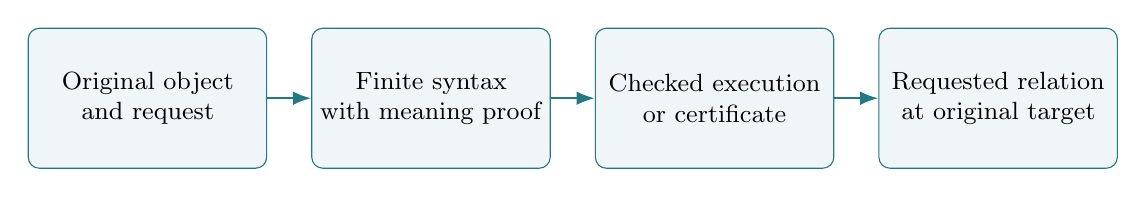
\begin{tikzpicture}[node distance=.22in, every node/.style={font=\small},
box/.style={draw=accent,rounded corners,fill=pale,text width=1.1in,
minimum height=.7in,align=center},arr/.style={-{Latex},thick,draw=accent}]
\node[box] (a) {Original object\\and request};
\node[box,right=of a] (b) {Finite syntax\\with meaning proof};
\node[box,right=of b] (c) {Checked execution\\or certificate};
\node[box,right=of c] (d) {Requested relation\\at original target};
\draw[arr] (a)--(b);\draw[arr] (b)--(c);\draw[arr] (c)--(d);
\end{tikzpicture}
\end{center}

\subsection{Keep computation out of definitional equality initially}
Definitional equality is the conversion relation used throughout elaboration
and type checking. Adding broad CAS normalization there would make ordinary
checking depend on expensive, domain-sensitive computation and complicate both
predictability and trust. The proposed computations should initially produce
ordinary theorems at explicit request boundaries. A result can then rewrite a
goal through a proof, leaving foundational conversion rules unchanged.

This is also a maintenance advantage. A changed heuristic can produce a
different certificate or fail to find one without changing what counts as the
same type throughout the language. Logical interfaces should be stable before
search policy is made ambitious.

\subsection{What the additional Lean experiments establish}\label{sec:secondarylean}
The secondary synthesis contributes useful executed probes on Lean 4.32.0 and
the same pinned mathlib revision as this report's original focused checks
\cite[\S7]{secondary}. It resolves concrete library declarations for local
derivative transfer, formal-series coefficients and truncation, square-root
branches, guarded casts, and finite reindexing. These are useful starting points
for wrappers. A successful \texttt{\#check} establishes that a declaration with
the printed type exists; it does not show that every proposed wrapper has all
the required hypotheses or that the full workflow is implemented.

Two existing tactics deserve explicit controls in the prototype:
\texttt{linear\_combination}, which reconstructs a polynomial combination,
and \texttt{grobner}, which closes the supplied polynomial consequence example.
The latter is a Lean-core tactic wrapping the ring component of \texttt{grind},
with resource limits; it is not evidence of an unrestricted complete
decision service. At the inspected revision, its default configuration includes
100,000 ring steps and a maximum ring degree of 1,024. Proof-producing success
is useful; failure under these limits is not a refutation. The claim
that none of the nine reports noticed it is also inaccurate: Cadence explicitly
names it in \S6.4, and Concord in \S5.6. The useful correction is that the
proposals did not exercise this existing tactic in Lean.

The noncomputability probe also needs a narrow reading. Failure to compile a
particular evaluation of a semantic \texttt{Polynomial} operation motivates a
separate executable representation; it does not establish that every use of
\texttt{Polynomial} or \texttt{Finsupp} is incapable of computation. Choosing
checker data and proving its interpretation remain design decisions.

\textbf{A promising microbenchmark, with limited scope.} The secondary
\code{PolyCert.lean} defines dense integer polynomials as lists and checks
\[
 X^n-1=(1+X+\cdots+X^{n-1})(X-1).
\]
The retained profiler logs give approximately 1.01 and 2.66 seconds for the
degree-1280 \texttt{decide} tactic plus kernel check in two runs. This is
encouraging for that family. However, the proved proposition is that a particular
Boolean checker invocation returns true. The checker has no denotational
soundness theorem or source-reification bridge, so this is not yet a
kernel-verified ideal-membership theorem about arbitrary polynomial inputs.

This family multiplies an \(n\)-coefficient list by a fixed two-coefficient
factor. It does not benchmark general dense-by-dense or multivariate
multiplication and does not support the report's quadratic-scaling inference.
Nor do these few observations establish negligible checking cost for all worked
examples. Measure coefficient size, sparsity, number of variables, certificate
length, elaboration, kernel checking, and startup separately before setting a
performance threshold. The imported timings remain historical observations,
not fresh measurements made by this revision.

The native-evaluation comparison has a clearer trust implication: the printed
axiom inventory contains a computation-specific native-evaluation axiom, whereas
the inspected \texttt{decide} examples do not add such an axiom. In the small
benchmark family, the native route is often slower than direct checking, but
the profiler logs do not establish a universal one-second compilation overhead.
This motivates
measuring both routes; it does not make speed alone sufficient to authorize a
different trust policy. Inspect transitive axiom dependencies under a
version-specific policy rather than blacklisting one historical constant name.

\decision{Make one checker's soundness theorem, interpretation of its finite
data, and original-target reconstruction the first new verified artifacts.
Use existing Lean tactics as controls. Treat the microbenchmark as evidence
that a small prototype is worth attempting, not as a completed feasibility
study of the proposed CAS.}

A fresh focused run for this revision checks the same rational polynomial
consequence using \texttt{grobner} and \texttt{linear\_combination}, and compares
the axiom inventories of a direct \texttt{decide} proof and a
\texttt{native\_decide} proof. It exits successfully. The two algebraic proofs
use the standard three axioms; in this imported environment the direct decision
proof uses \texttt{propext}, while the native proof additionally uses its
computation-specific axiom. The retained receipt records this actual difference;
it does not copy the no-import probe's empty inventory into a different environment.

\section{Worked case I: guards, domains, and complete answers}\label{sec:guards}
The small rational identity
\[
 \frac{x^2-1}{x-1}=x+1
\]
is an unusually effective language test. As an equality of real expressions
using total division, it needs \(x\ne1\). At \(x=1\), the left side is zero
and the right side is two. As an equality of rational functions, it has a
different interpretation. As equality of partial functions, both values and
domains must be compared. A frontend must not slide between these meanings
because they share a familiar printed fraction.

The correct global total-function identity is piecewise:
\[
 \frac{x^2-1}{x-1}=
 \begin{cases}0,&x=1,\\x+1,&x\ne1.\end{cases}
\]
An interface can offer a conditional equality, this global piecewise result, or
a domain-restricted transformation, depending on the request. Those are
different mathematical answers with different usefulness. Noema's prototype
models retention of the original denominators and rejection of a certificate
with substituted guards; Cadence, Meridian, and Vantage generalize the
distinction to guarded computation and coverage
\cite[\S\S5--6,11.1]{noema}\cite{cadence,meridian,vantage}.

The choice of default semantics is therefore visible in solving, not merely in
notation. Over \(\R\), the equation \((x^2-1)/(x-1)=0\) has solution set
\(\{-1,1\}\) with Lean's total division and \(\{-1\}\) with the denominator
excluded by partial-expression semantics. The secondary synthesis is right to
make that default an explicit interface decision \cite[\S6.1]{secondary}.
Existing total Lean statements must retain their meaning when lifted; an
opt-in partial-expression package should state its domain in the request.

Complete solving adds a second dimension. Over a field, the equation \(ax=b\)
has the following complete description:
\[
 \{x:ax=b\}=
 \begin{cases}
 \{b/a\},&a\ne0,\\
 \text{the entire field},&a=0\text{ and }b=0,\\
 \varnothing,&a=0\text{ and }b\ne0.
 \end{cases}
\]
Verifying \(b/a\) under \(a\ne0\) is witness correctness. Proving the displayed
classification requires soundness and coverage for all branches. A generic
solution formula cannot be specialized to \(a=0\) as though the original
nonzero guard had vanished. A \emph{solution predicate} is often the right
semantic interface, because some solution sets are infinite and cannot be
represented by a finite list.

Branch selection appears even in elementary radical denesting:
\[
 \sqrt{5+2\sqrt6}=\sqrt3+\sqrt2.
\]
The square identity is necessary, but the nonnegative branch condition is also
needed. The negative of the proposed right side has the same square and is
therefore an excellent malformed candidate. Similarly, isolating the positive
root of \(x^2-2\) does not describe all roots, and a real square-root statement
does not automatically transfer to a complex principal-branch statement.

\decision{Implement the guarantee selector as a mathematical part of the
request: equality on this domain, one witness, or a complete solution
predicate. Let computation supply candidates, and make a weaker answer visible
as a different result that cannot discharge the stronger request.}

\section{Worked case II: exact finite information about an infinite object}\label{sec:jets}
Let \(R[[t]]\) denote formal power series over a commutative ring \(R\). Write
\[
 A\equiv_N B\quad\Longleftrightarrow\quad
       [t^k]A=[t^k]B\quad\text{for all }k<N.
\]
Equivalently, \(A-B\) belongs to the ideal \((t^N)\). This is exact finite
information, often called a jet. It is not a floating approximation, an analytic
big-O statement, or an assertion that the full series are equal.

Addition and multiplication preserve the minimum available precision.
Differentiation generally consumes one order: input precision \(N+1\) suffices
for output precision \(N\). For example, \(t\) and \(t+t^3\) agree below
degree three over \(\Q\), while their derivatives differ at degree two.
Substitution has its own side conditions; substituting a series with nonzero
constant term into an arbitrary formal series is not generally defined by
finite coefficient sums. Precision planning must invoke the appropriate
operation theorem, not apply one universal arithmetic rule.

\Needspace{14\baselineskip}
\subsection{A general residual-to-jet theorem}
The following theorem captures Locus's central idea and makes its hypotheses
explicit \cite[formal-root development]{locus}.

\begin{proposition}\label{prop:residual}
Let \(F(Y)\in R[[t]][Y]\), and let \(\Delta\in R[[t]]\) satisfy
\(F(\Delta)=0\) and \(\Delta(0)=d\). Reduce the coefficients of \(F\) modulo
\(t\) to obtain \(\overline F\in R[Y]\). Assume
\(\overline F'(d)\) is a unit in \(R\). If \(N\ge1\), \(J(0)=d\), and
\(F(J)\equiv_N0\), then \(J\equiv_N\Delta\).
\end{proposition}
\begin{proof}
Polynomial subtraction factors as
\[
 F(J)-F(\Delta)=(J-\Delta)U
\]
for a series \(U\). Because \(J\) and \(\Delta\) have the same constant term,
\(U(0)=\overline F'(d)\). A formal series with unit constant coefficient is a
unit. Thus \(J-\Delta=F(J)U^{-1}\) belongs to \((t^N)\).
\end{proof}

No field assumption is needed. Conversely, ``nonzero'' cannot replace ``unit''
over an arbitrary ring. In \(R=\Z/4\Z\), take \(F(Y)=2Y\), \(\Delta=0\),
and \(J=2t\). The residual is exactly zero and the derivative is the nonzero
element \(2\), but \(J\not\equiv_2\Delta\). A theorem wrapper that forgets
the unit condition would admit a false observation.

The theorem is relative to an \emph{existing} root. It neither constructs that
root nor proves its existence. This is a feature: an author can retain an
arbitrary \(\Delta\) from a theorem statement while a finite checker computes
information about it. A separate existence theorem can be supplied when the
task actually introduces a new root.

\subsection{A concrete dyadic germ}
Take the rational formal series specified by
\[
 \Delta+4\Delta^2=\frac49t,\qquad \Delta(0)=0.
\]
Writing \(\Delta=\sum_{n\ge1}a_nt^n\) gives
\[
 a_1=\frac49,\qquad
 a_n=-4\sum_{i=1}^{n-1}a_i a_{n-i}\quad(n\ge2).
\]
The first five coefficients give
\[
 J=\frac49t-\frac{64}{81}t^2+\frac{2048}{729}t^3
       -\frac{81920}{6561}t^4+\frac{3670016}{59049}t^5.
\]
A rational polynomial checker can establish that
\(J+4J^2-4t/9\) has zero coefficients below degree six. The derivative of the
defining polynomial at the constant term is \(1\), hence a unit.
Proposition~\ref{prop:residual} then gives \(J\equiv_6\Delta\). The checker's
job is finite arithmetic; the library theorem handles the infinite object.
The coefficient formula
\[
 a_n=(-1)^{n-1}\frac{4^{2n-1}}{9^n}C_{n-1},\qquad n\ge1,
\]
where \(C_m\) is the \(m\)-th Catalan number, is a separate universal result
obtainable from the recurrence. Checking the first five coefficients does not
prove that formula for every \(n\).

Newton refinement fits the same contract. If \(F'(J)\) is a unit and
\(F(J)\in(t^N)\), put \(h=-F(J)/F'(J)\). Then \(h\in(t^N)\), and the
polynomial identity
\[
 F(J+h)=F(J)+F'(J)h+h^2H
\]
shows the new residual lies in \((t^{2N})\). A finite implementation still
needs a proof that its truncations and inverse computation realize these
operations to the advertised precision. The algebraic doubling argument does
not supply that execution proof automatically.

\subsection{A distinct route: precision-improving fixed points}
Concord uses a related but different mechanism \cite[\S7.3]{concord}. Over a commutative
\(\Q\)-algebra, let \(\Psi(S)=z\exp(-aS)\) on zero-constant formal series.
If \(S\equiv_kT\), then \(\Psi(S)\equiv_{k+1}\Psi(T)\). For an arbitrary
fixed point \(T=\Psi(T)\), a candidate \(P\) with zero constant term and
\(P-\Psi(P)\equiv_N0\) therefore satisfies \(P\equiv_NT\): start with
constant-term agreement and improve it one order at a time up to \(N\).
For instance,
\[
 P=z-az^2+\frac32a^2z^3-\frac83a^3z^4
\]
is the expected observation below degree five. This is a contraction argument
in formal precision, not a numerical convergence theorem. It illustrates why a
general observation interface should admit multiple mathematically certified
routes without forcing them into one algorithm.

\decision{Use residual-to-observation as the first nontrivial bridge between a
CAS and an arbitrary semantic object. Keep precision in the type of the result,
and evaluate demand-driven precision as a separate optimization with its own
correctness and performance measurements.}

\section{Worked case III: algebraic generality and symbolic calculus}\label{sec:generality}
Conciseness should not be purchased by silently strengthening hypotheses. A
computer algebra routine may prefer fields, while the theorem being proved is
about an additive group or a ring with zero divisors. The language needs to
preserve that distinction and make legitimate transport reusable.

\subsection{Binomial inversion and quantifier scope}
For sequences in an additive commutative group, define the binomial transform
using integer scalar action. The correct inversion statement is
\begin{align*}
 &\left(\forall n,\quad b_n=\sum_{k=0}^n\binom nk\,\boldsymbol{\cdot}\,a_k\right)\\
 &\hspace{.35in}\Longleftrightarrow
 \left(\forall n,\quad a_n=\sum_{k=0}^n
       (-1)^{n-k}\binom nk\,\boldsymbol{\cdot}\,b_k\right).
\end{align*}
Here the bold dot means scalar action, not multiplication of two elements of the
group. The scalar orthogonality identity is proved over \(\Z\), then applied
through distributivity and finite-sum rearrangement. No field structure on the
sequence values is needed.

The scope of \(\forall n\) matters. At a single fixed index, the displayed
forward equality does not imply the inverse equality at that index, because
the latter depends on earlier rows. Take \(n=1\), \(a_0=a_1=0\), \(b_0=1\),
and \(b_1=0\). The forward row says \(0=0\); the inverse row would say
\(0=-1\). Cadence's and Concord's compact displays need to be read with the
uniform sequence-level quantification supplied by their surrounding argument
\cite[\S8.3]{cadence}\cite[\S8.3]{concord}. The focused Lean examples in the
evidence package check both the valid forward row and failure of its supposed
pointwise inverse.

This is a statement-interface issue as much as a theorem issue. A compact
renderer that moves or hides a quantifier can change the claim. The statement
seal should expose the uniform scope, while the method interface records that
all lower-index equations are available to the inversion proof.

\subsection{Transport is a theorem about a particular relation}
A polynomial identity over \(\Q\) evaluates correctly in every commutative
\(\Q\)-algebra, including the dual-number ring \(\Q[\varepsilon]/(\varepsilon^2)\).
The forward preservation theorem does not require an injective scalar map.
Thus a universal polynomial computation can support a theorem with zero
divisors, provided its certificate uses only valid rational-algebra operations.
Trying a few rational substitutions does not establish that universal identity.

Reflection is a different direction. An injective map can reflect equality of
mapped elements, but not every statement about a richer target structure. For
example, \(X\) belongs to the ideal generated by \(2X\) in \(\Q[X]\), using
the multiplier \(1/2\). It does not belong to the corresponding ideal in
\(\Z[X]\): the coefficient of \(X\) in \(2Xh(X)\) is even for every integer
polynomial \(h\). The embedding \(\Z\hookrightarrow\Q\) is injective; the
witness domain has nonetheless expanded. A representation registry must attach
transport theorems to individual relations rather than advertise a universal
``safe coercion'' flag.

The formal Abel identity illustrates the positive opportunity. If an arbitrary
zero-constant series satisfies \(T=z\exp(-aT)\), then over a commutative
\(\Q\)-algebra the normalized exponential-generating-function observation is
\[
 n!\,[z^n]\exp(xT)=x(x-na)^{n-1}\qquad(n\ge1),
\]
with constant coefficient \(1\). A universal coefficient theorem and polynomial
transport can establish this under general hypotheses. A finite jet of one
canonical solution cannot establish it for every \(n\) and every originally
quantified solution. Facet and Concord are particularly useful on that object
identity boundary; Vantage develops normalized EGF observations into a broader
definition interface \cite{facet,concord,vantage}.

\subsection{A symbolic derivative family with local hypotheses}
Meridian and Prism develop a stronger example than evaluating a few derivatives
\cite[Lambert derivative developments]{meridian,prism}. Let
\[
 P_0(w)=1,\qquad
 P_{n+1}(w)=(1+w)P_n'(w)-\bigl((n+1)w+3n+2\bigr)P_n(w),
\]
so every \(P_n\) is an integer polynomial. The first terms are
\begin{align*}
 P_1(w)&=-w-2,\\
 P_2(w)&=2w^2+8w+9,\\
 P_3(w)&=-6w^3-36w^2-79w-64.
\end{align*}
Set
\[
 H_n(w)=\frac{e^{-(n+1)w}P_n(w)}{(1+w)^{2n+1}},\qquad
 \phi(w)=\frac{e^{-w}}{1+w}.
\]
For \(w\ne-1\), the product and quotient rules give
\[
 H_n'(w)\phi(w)=H_{n+1}(w).
\]
The displayed recurrence is exactly the polynomial numerator remaining after
common factors are extracted. Its index starts at zero here; some source
presentations shift the polynomial index by one.

Suppose \(U\subseteq\R\) is open and \(W:\R\to\R\) has derivative
\(\phi(W(x))\) at every \(x\in U\), with \(W(x)\ne-1\) there. Then
\[
 W^{(n+1)}(x)=H_n(W(x))\qquad(x\in U)
\]
follows by induction, using the chain rule on the entire open set. Derivative
existence is part of the hypothesis and induction, not inferred from an
equation involving a totalized derivative operator alone. The condition
\(W(x)\ne-1\) is the relevant pole exclusion; imposing \(W(x)>-1\) would
needlessly exclude another real branch in applicable settings.

The neighborhood condition is essential. Two functions can agree at a point
and have different derivatives there: \(f(x)=x\) and \(g(x)=0\) agree at zero.
An induction hypothesis valid on \(U\), together with openness, yields the
local equality needed to differentiate. A proof method should package this
analytic plumbing as an ordinary theorem, while the computation service
certifies the polynomial recurrence. Checking only \(P_0,\ldots,P_3\) does
not prove the arbitrary-index recurrence or the analytic induction.

The underlying recurrence and analytic argument are attributed by the proposals
to existing ProveIt work. The language contribution is a usable interface
between a computable finite representation and the general theorem, not a claim
to have discovered the mathematical family. This makes a good staged integration test
after a smaller polynomial and formal-jet slice is working.

\subsection{A small specification gap with a useful lesson}
Vantage's illustrative telescoping contract should make its range convention
explicit. For inclusive natural intervals and \(a\le b\),
\[
 \sum_{k=a}^{b}\bigl(G(k+1)-G(k)\bigr)=G(b+1)-G(a).
\]
If \(a=3\), \(b=1\), and \(G(k)=k\) in \(\Z\), the sum is empty and
equals zero, while the displayed right side is \(-1\). An ordered-range
premise or a correct empty-range branch is needed
\cite[\S10.4]{vantage}. This is a gap in an illustrative proposed contract,
not an implemented checker defect. Such tiny negative neighbors often test a
language's semantic discipline better than another successful long example.

\section{Leant, proof providers, and negative evidence}\label{sec:leant}
The user's Leant work on automatic term synthesis and tactic suggestion is
directly relevant to this architecture. The earlier source review distinguishes
search over a restricted term language from Lean-side acceptance, and distinguishes
a successful search invocation from successful replay of the text shown to the
user \cite{round1,claude}. The second-round proposals largely accept those
boundaries and extend them to CAS and counterexample providers. The analysis
below is a proposed integration contract, not a claim that the current external
Leant checkout already implements every field.

\subsection{A provider supplies candidates for an exact request}
A request should carry, or refer unambiguously to, the elaborated target,
ordered local context, universe and instance information, relevant environment
identity, source revision, and policy. A provider may search using a simpler
internal representation, but an accepted proof must reconstruct at that exact
request. A hash helps identify a request; it is not a proof that the encoded
context faithfully represents the caller's semantics.

The provider can return a candidate term, a tactic edit, a certificate, an
explicitly conditional result, or no result. These should be decoded through a
versioned protocol rather than inferred from a suggestive log line. Resource
exhaustion and unsupported input deserve distinct diagnostic explanations even
when neither produces mathematical evidence.

For a tactic suggestion, retain three separate receipts:
\begin{enumerate}
\item The search or synthesis operation produced a candidate under the stated
request and budget.
\item The proposed tactic or term elaborated at the exact target with the
required completion and axiom policy.
\item The actual displayed edit was inserted transactionally into the source
and replayed successfully in its surrounding context.
\end{enumerate}
The third receipt matters because formatting, name resolution, comments,
indentation, or a shortened suggestion can make the displayed edit differ from
the successful internal action. A failed attempt must restore metavariable and
source state before another candidate is tried. Retaining a term cannot excuse
a broken advertised edit; retaining a working edit cannot excuse a changed goal.

\subsection{Why complete search failure is still not negation}
Even a complete search for a specified calculus reports a judgment about that
calculus. It does not automatically prove a negation in Lean. A simple example,
emphasized by Vantage, is the schema \(P\lor\neg P\): it is not uniformly
derivable in intuitionistic propositional logic, yet intuitionistic reasoning
proves
\[
 \neg\neg(P\lor\neg P).
\]
Indeed, assuming \(h:\neg(P\lor\neg P)\), any proof of \(P\) contradicts
\(h\), so \(\neg P\); that right-hand disjunct then also contradicts \(h\).
Thus the lack of an intuitionistic derivation cannot be reinterpreted as
\(\neg(P\lor\neg P)\). Classical Lean can prove the excluded-middle schema
under its classical assumptions \cite[\S5.7]{vantage}.

A provider may legitimately report ``not derivable in this calculus under these
assumptions,'' or supply a checked countermodel with a theorem connecting it to
the requested judgment. To refute an original Lean proposition \(Q\), it needs
an original-target proof of \(\neg Q\), or a proved adequacy bridge plus checked
evidence sufficient to construct that proof. An empty recorded list of abstracted
nodes is diagnostic metadata, not such a bridge. Nor does failure to synthesize a polymorphic
term of type \(\forall A, A\) mean that every individual \(A\) is empty.

This distinction should affect interface wording. ``No candidate within this
budget,'' ``unsupported target,'' ``not derivable in the stated calculus,'' and
``proved false'' are useful different outcomes. The UI need not expose internal
search machinery to every author, but it must not display a stronger
mathematical conclusion than the evidence supports.

\subsection{Term synthesis and CAS can share an acceptance boundary}
The common provider abstraction is not ``a service that returns proofs.'' It is
``a service that proposes data and evidence for a typed request.'' A term
synthesizer proposes an inhabitant; a CAS proposes a normal form and certificate;
a counterexample searcher proposes a witness refuting a statement. The same
original-target validation, transaction isolation, provenance, resource
accounting, and retained replay rules can apply to all three.

This does not imply one universal certificate language. The mathematical
soundness theorem remains specific to each provider and guarantee. A shared
envelope reduces duplicated integration work; a shared untyped notion of
success would erase exactly the distinctions the reports have clarified.

\section{Decisions still open, and refinements proposed here}\label{sec:decisions}
The papers differ more in implementation strategy than in foundational logic.
The following choices deserve explicit decisions rather than another layer of
compatible terminology.

\begin{center}\small
\begin{tabularx}{\textwidth}{@{}P{1.25in}Y Y@{}}
\toprule
Choice & Main benefit & Main unresolved cost\\
\midrule
Guarded algebra first & Small checkers; cancellation and complete linear solving
expose semantic mistakes immediately. & May show service and library value
without establishing a need for new syntax.\\
Formal-root jets first & Demonstrates computation about an arbitrary infinite
object through a compact generic theorem. & Needs formal-series interfaces,
precision contracts, and a verified finite representation.\\
Symbolic calculus first & Tests arbitrary indices, local hypotheses, and
representation transport together. & Too many moving parts can obscure which
component failed or improved usability.\\
Rich definition interface first & Attacks the cost of introducing reusable
objects and observations, including EGF packages. & A broad schema language
risks preceding evidence about common definition patterns.\\
Document view first & Can test comprehension and statement visibility using
existing Lean input. & May leave the authoring burden largely unchanged.\\
New input form first & Directly tests concise mathematical authoring. & Requires
an additional interpretation and repair surface before benefits are known.\\
\bottomrule
\end{tabularx}
\end{center}

\subsection{Account for what Lean's workspace already supplies}\label{sec:workspace}
The secondary synthesis asks a useful question that deserves an explicit answer:
which parts of the proposed persistent mathematical workspace are new, and
which merely record state Lean already maintains \cite[\S8.2]{secondary}?
The first implementation should start with the following allocation.

\begin{center}\small
\begin{tabularx}{\textwidth}{@{}P{1.4in}Y Y@{}}
\toprule
Need & Existing Lean mechanism & Additional layer to justify\\
\midrule
Local parameters and hypotheses & Sections, variables, and the elaborator's
local context & A readable record of dependencies and interpretation.\\
Local facts and intermediate claims & \texttt{have} declarations and proof terms
& Method roles, explanation, and source-to-evidence mapping.\\
Structures and local conventions & Instances, local notation, and explicit
arguments & Notices when resolution changes mathematical meaning.\\
Routine proof search & Tactics and controlled simplification sets & Named
profiles, budgets, provenance, and stable replay evidence.\\
Alternative computational views & Definitions and transport theorems & An
object-indexed registry of accepted observations, guards, and selected routes.\\
Editing and reuse & Elaborator snapshots and ordinary source checking &
Transactional result acceptance, origin checks, and migration receipts.\\
\bottomrule
\end{tabularx}
\end{center}

The purpose is not to replace Lean's context management. Store additional state
only when it enables a specified operation that ordinary Lean and its editor do
not already expose sufficiently: explaining a generated guard, replaying a
published computation, or invalidating an observation after its origin changes.
This mapping should be part of the baseline comparison, so a large new registry
cannot claim credit for work already done by local contexts and proof terms.

\subsection{Reuse evidence through explicit entailment}
Generalizing the reports' observation-weakening rules
\cite[\S7.4]{concord}\cite[\S4.3]{cadence}, this synthesis recommends an explicit
reuse rule beyond exact hash matching or an informal claim that one result is
``stronger.'' A retained
certificate may be reused when a checked adapter shows that the current request
follows from its guarantee: the current context proves its guards, the semantic
object correspondence is established, and the retained relation entails the
requested relation under the current policy.

Different coordinates have different variance. Higher jet precision can answer
a lower-precision request. Equality on a larger domain can answer one on a
smaller domain. A narrower interval can answer a wider enclosure request.
Stronger assumptions make a theorem less broadly applicable, not more.
Additional axioms may violate the new project's trust policy even when the
proposition is identical. The adapter should prove these individual entailments
rather than squeeze them into a single rank.

Exact identity remains an efficient fast path. Entailment-based reuse is an
optional extension whose benefit must exceed proof and cache complexity. It
should not be used to hide a changed statement during source editing.

\subsection{Make the visible obligations sufficient to interpret the claim}
Readable mathematics requires compression. The right question is which
information may be collapsed without misleading the reader. I propose a
\emph{visible obligation boundary}: the default rendering must expose unresolved
conditions and accepted distinctions that affect the claim's domain, branch,
precision, completeness, or trust policy. Routine proofs behind those conditions
can be folded away while remaining inspectable.

This is a rendering contract against the typed evidence graph, not an assertion
that there is an easily computable minimal display. A finite-jet result should
show its precision; a conditional equality should show its condition; a root
selection should show which root is selected. An expanded view can explain why
those conditions suffice. Testing whether readers reconstruct the intended
claim is more informative than counting visible lines alone.

\subsection{Keep status dimensions separate}
An implementation can avoid an unwieldy enumeration of every possible result
by separating: proof validation status; unresolved guards; guarantee kind;
source/provenance binding; and policy compatibility. A fully checked theorem
\(G\to Q\) may still have an unresolved guard \(G\) at the caller. A valid
finite observation may still fail a request for exact equality. A proved result
may still need source-edit replay. These are ordinary, explainable states rather
than exceptions to a binary success badge.

\subsection{Route changes should be meaningful edits}
Changing an internal polynomial normalization algorithm need not prompt the
author if the requested relation, object, and accepted policy remain fixed and
the result rechecks. Changing a branch, witness, domain, method explanation, or
public theorem dependency can affect mathematical meaning or maintainability.
Such changes should be reported at the level of the resulting statement or
argument. A blanket ban on automatic choices would defeat the goal of synthesis;
invisible semantic changes would defeat its reliability.

Coherence is therefore relative to what the request observes. Two exact
presentations can be coherent through their shared object. Two valid intervals
need not have identical endpoints. Two proofs of a proposition may be
interchangeable for kernel acceptance but differ as explanations of the
author's chosen method. Logical equivalence alone does not settle every
editorial policy.

\section{A discriminating implementation and evaluation plan}\label{sec:evaluation}
The next iteration should produce one shared protocol and a small complete
workflow. Nine more surface grammars would add less information than one
experiment that reveals which layer actually saves effort.

\subsection{Stage one: a checked computation request}
Implement a typed request with source binding, a mathematical guarantee, and
scoped guards. Supply an ordinary Lean theorem interface and a finite integer
or rational polynomial representation with proved interpretation and checker
soundness. Exercise guarded cancellation and all-parameter \(ax=b\). Accept a
proof only through the actual execution route selected by the project's trust
policy. Retain evidence and replay it after disabling the discovery service.
Following the useful priority in \emph{Nine Workbenches}, prove the first
checker's denotational soundness theorem and original-expression reconstruction
before adding a second checker or a new grammar \cite[\S\S9.3--10]{secondary}.
Include \texttt{linear\_combination} and the bounded \texttt{grobner} tactic as
existing proof-producing controls, with their actual contracts documented.

The exit gate is an end-to-end demonstration, not a large example count: the
original source request elaborates, the producer is untrusted, malformed
certificates are rejected at the correct boundary, the accepted result has the
advertised domain and completeness, and saved evidence rechecks without search.
Document checker time, certificate size, reification time, and dependency cost.

\subsection{Stage two: a fixed object and a finite observation}
Implement Proposition~\ref{prop:residual} and an executable truncated-polynomial
checker for the dyadic germ. The theorem statement must quantify the original
\(\Delta\); the computed \(J\) supplies only the requested jet. Demonstrate
changing the requested precision, changing the producer, and rejecting a
nonunit derivative hypothesis in a generalized ring example. Measure where
full normalization, certificates, and demand-driven truncation differ in cost.

Use the same service from ordinary Lean and a small mathematical interface.
This is the first strong test of whether a new authoring layer improves
understanding beyond what the theorem package alone achieves. Keep the initial
definition package small: semantic object, defining equation, observations,
and the specific transport theorems used in the experiment.

\subsection{Stage three: semantic integration and a held-out task}
Add the symbolic derivative family from Section~\ref{sec:generality}, or an
equally demanding case selected before implementation. This tests locality,
arbitrary indices, and algebraic representation without merely replaying the
first example. Reserve an additional, previously unseen related theorem for the
held-out evaluation; a case used to design the system is not held out.
The secondary synthesis's ``fourth-file rule'' provides a concrete way to seek
new examples: choose a source file no earlier report discussed. That makes it
development material once inspected, so reserve a separate sealed task for the
actual held-out measurement. Already-discussed Bell and Abel files cannot serve
as unseen tests of a design built around them.
Include a definition-interface task such as normalized EGF
coefficients and a task involving a complete solution predicate.

Apply controlled edits: rename a wrapper role, change a theorem's hypotheses,
alter a branch condition, move a proof step into another scope, change a
routine profile, and upgrade a dependency. Record which edits preserve a
certificate, which require a checked adapter, and which require new discovery.
Do not count automatic repair as successful until the resulting statement,
explanation, and actual source replay have been checked.

Include a toolchain migration that changes the native-evaluation axiom scheme.
Compare dependencies against the destination version's explicit trust policy,
recheck retained evidence there, and issue a new receipt. Renaming an axiom in
an allowlist is not a substitute for revalidation. Losing a discovery service
must not prevent strict replay of evidence already accepted and retained.

\subsection{Separate the effects of syntax, libraries, and services}
At minimum compare four treatments:
\begin{enumerate}
\item ordinary Lean with the existing library;
\item Lean with the new theorem and definition packages;
\item Lean with those packages and the same computation/provider service;
\item the proposed mathematical frontend with exactly those packages and service.
\end{enumerate}
A rendered document view can be an additional ablation rather than a different
backend. Match training time, solver budgets, and available hints. Include
authors other than the designers. Report startup learning cost separately from
repeated use, and preserve unsuccessful attempts rather than measuring only
finished proofs. For Leant, collect the obligations generated by these
computations and distinguish single-lemma lookup from genuine structural
composition. Compare the same obligations with and without Leant under matched
budgets; the value of a generic synthesizer elsewhere does not establish its
value for the CAS workflow. This experiment can begin before a complete
source-edit interface exists.

Useful outcomes include time to a correctly stated checked theorem; author
edits and interventions; maintenance time after a controlled change; reader
accuracy about the actual claim; and all amortized infrastructure work.
Visible token count can describe presentation, but should not serve as the
primary success metric. A ten-line proof that hides the wrong domain has not
improved mathematical expression.

\subsection{A blind semantic-reading test}
Before readers see the expanded evidence, ask them to reconstruct the guarantee
of a compact result: the quantified object, domain, branch, precision,
completeness, and unresolved conditions. Use matched positive and negative
neighbors with equally plausible formatting. Compare their answers with the
elaborated specification, then reveal the expanded view and measure whether it
resolves mistakes. This directly tests whether concise notation communicates
mathematics rather than merely looking familiar.

\begin{center}\small
\begin{tabularx}{\textwidth}{@{}P{1.5in}Y@{}}
\toprule
Negative neighbor & Required system behavior\\
\midrule
Cancellation at the pole & Reject unconditional equality; preserve the guard
or supply a checked piecewise result.\\
Specialize \(ax=b\) at \(a=0\) & Recompute branch coverage; do not reuse the
generic singleton as a complete answer.\\
Differentiate a finite jet & Require enough input precision and actual local
analytic hypotheses when differentiating functions.\\
Nonunit formal derivative & Refuse the residual-to-jet theorem unless its unit
premise is established.\\
One binomial row & Refuse the sequence inversion method without all required
rows or an appropriate uniform hypothesis.\\
Integer ideal via rational witness & Refuse backward transport without a
relation-specific theorem.\\
Wrong radical sign & Reject the candidate despite the matching square.\\
Reversed telescoping bounds & Use a proved empty-range case or reject the
ordered-range method.\\
Stale target or sibling scope & Reject evidence at the request-binding boundary.\\
Successful search, broken displayed edit & Keep the source unchanged and report
that edit replay failed.\\
Complete abstract search failure & Report the calculus-level outcome; do not
manufacture an original-target negation.\\
\bottomrule
\end{tabularx}
\end{center}

\subsection{Turn the negative catalogue into paired executable cases}
The secondary synthesis consolidates the source suites into 51 canonical
mutations with per-report row identifiers \cite[\S9.2]{secondary}. This is a
useful shared backlog. Reproducing its data establishes 183 report--mutation
incidences, covering 182 distinct original table rows; the former number should
not be described as the number of original tests. A source row can also cover
more than one canonical mutation. Ten categories occur in at least seven
suites, and 17 in at least five. These are editorial classifications of proposed
tests, not 51 executed tests or a measure of their relative severity.

For each implemented category, retain a positive neighbor, the mutated input,
the expected mathematical outcome, the precise rejection boundary, and the
observed diagnostic. A system that rejects both cases must fail the test.
Frequency is useful for selecting shared examples, but a rare mutation such as
swapping dependent quantifiers can expose a more serious bug than a common
arithmetic error. Preserve the complete catalogue and prioritize by the first
slice's contracts and plausible failure modes.

Preserve the exact subcases inside a consolidated category. For example, the
catalogue groups cancellation and inversion failures together: a regular element
may be cancelled from an equality, but constructing its multiplicative inverse
requires a unit. The integer \(2\) is regular and not a unit. A shared category
name must not erase that difference in the required theorem.

Add the three bridge-registry cases in Section~\ref{sec:bridges} as tests of the
interface specification itself, together with the circular-guard case in which
a result is improperly used to establish its own prerequisite. Keep a valid
degenerate enclosure as a positive case: rejecting every proposed transition
from bounds to equality would hide an overly restrictive contract rather than
demonstrate soundness.

\subsection{Choose thresholds before the main study}
The reports agree on measurement but do not establish numeric success thresholds.
Set those after a small pilot determines task variance and before evaluating
the main comparison. Report paired results and uncertainty, not just averages.
Predeclare a practical improvement target, acceptable semantic-reading error,
checking-cost limits, and an infrastructure amortization horizon.

Stop or reduce the language layer if package and service improvements explain
the observed gains, if readers systematically mistake weaker guarantees for
stronger ones, or if maintenance cost exceeds the saved author effort. A
successful Lean library, provider protocol, and linter can be the right result.
This stopping rule protects the mathematical objective from commitment to a
particular syntax or project identity.

\clearpage
\section{Questions for the next discussion}\label{sec:questions}
The following questions are intended to produce decisions or experiments. They
are not requests to answer every architectural detail before coding.
\begin{enumerate}[label=\textbf{Q\arabic*.},itemsep=.7em]
\item \textbf{Which first task must work from authored source to retained proof?}
Choose guarded cancellation and complete linear solving as the smallest slice,
or the formal-root jet as the distinctive slice. Name the exact theorem,
negative neighbor, and replay artifact required for completion.

\item \textbf{What must every request say about its result?} Decide the initial
guarantee vocabulary: equality, equality on a domain, finite jet, witness, and
complete solution predicate are enough to expose most current disagreements.
Which can be inferred without surprising the author? How will requests select
total operations or opt-in partial-expression semantics?

\item \textbf{What is the initial trusted execution route?} Select one route
for polynomial checking, state its pinned axioms and runtime dependencies, and
measure reification and proof checking separately from candidate discovery.
What additional benefit must a new checker demonstrate against
\texttt{linear\_combination} and the bounded \texttt{grobner} tactic?

\item \textbf{What can an author delegate by specification?} Distinguish choosing
a witness that satisfies a fixed request from changing the requested object,
branch, domain, or proof explanation. Which changes require a visible notice,
and what evidence allows the notice to be dismissed?

\item \textbf{How much of a conditional result is visible by default?} Use the
blind reading experiment to decide whether a collapsed guard badge, inline
condition, or case split communicates the actual claim reliably.

\item \textbf{What representation changes are automatic?} Begin with exact
presentations and requested observations of a fixed object. Decide whether the
first version pins routes, permits certified coherent alternatives, or supports
entailment-based certificate reuse across changed requests. Which workspace
fields are new metadata, and which expose existing Lean context mechanisms?

\item \textbf{What precisely can Leant report negatively?} Specify protocol
outcomes for unsupported input, bounded failure, complete calculus
nonderivability, and checked original-target refutation. Identify the missing
adequacy theorem for any proposed promotion between them. Which actual
CAS-generated obligations benefit from composition rather than theorem lookup?

\item \textbf{Which definition interface is worth implementing first?} Compare
the formal-root package and normalized EGF observations. List the ordinary Lean
definitions and theorems each needs before choosing new declaration syntax.

\item \textbf{What evidence survives publication and migration?} Decide which
terms, certificates, source mappings, method explanations, and environment pins
are mandatory, and what an upgrade must recheck to produce a new receipt,
including an upgrade that changes native-evaluation axiom conventions.

\item \textbf{What result would persuade us to keep only the library and tools?}
Predeclare the fair Lean baseline, independent-reader task, maintenance edits,
cost accounting, and practical stopping threshold. This is the decision that
makes the next iteration an experiment rather than another advocacy document.
\end{enumerate}

\clearpage
\appendix
\section{Convergence crosswalk and source locators}\label{app:crosswalk}
The eight feature codes are defined in Section~\ref{sec:convergence}. Every cell
below is an \emph{explicit proposal}, not an implemented capability. Each cell
gives a representative printed section and one-based TeX source range. The
machine-readable \code{convergence.json} retains all 241 supporting references,
qualifications, and the feature definitions for the 72 cells. This compact table
is a reading aid, not a substitute for those qualifications.

% Generated from the first source reference of every convergence.json cell.
% Exactly 72 proposal-level cells; the full JSON retains all references and qualifications.
\begingroup
\small
\begin{longtable}{@{}P{.8in}P{2.45in}P{2.45in}@{}}
\toprule
Report & R/O/G/V source locators & D/L/P/E source locators\\
\midrule
\endfirsthead
\toprule
Report & R/O/G/V source locators & D/L/P/E source locators\\
\midrule
\endhead
\midrule
\multicolumn{3}{r}{\emph{Continued on next page}}\\
\endfoot
\bottomrule
\endlastfoot
\textbf{Accord} & \textbf{R}: \S{}6.1, lines 519--549 \newline
\textbf{O}: \S{}5.1, lines 409--420 \newline
\textbf{G}: \S{}8.1, lines 775--788 \newline
\textbf{V}: \S{}7.1, lines 612--648 &
\textbf{D}: \S{}5.1, lines 409--420 \newline
\textbf{L}: \S{}13.2, lines 1319--1346 \newline
\textbf{P}: \S{}14.3, lines 1448--1463 \newline
\textbf{E}: \S{}17.1, lines 1588--1600\\
\addlinespace[.65em]
\textbf{Cadence} & \textbf{R}: \S{}2.3, lines 286--301 \newline
\textbf{O}: \S{}5.1, lines 507--543 \newline
\textbf{G}: \S{}4.2, lines 434--449 \newline
\textbf{V}: \S{}6.2, lines 653--677 &
\textbf{D}: \S{}5.1, lines 507--529 \newline
\textbf{L}: \S{}12.2, lines 1325--1341 \newline
\textbf{P}: \S{}14.1, lines 1491--1510 \newline
\textbf{E}: \S{}16.1, lines 1611--1630\\
\addlinespace[.65em]
\textbf{Concord} & \textbf{R}: \S{}4.1, lines 252--280 \newline
\textbf{O}: \S{}6.1, lines 393--398 \newline
\textbf{G}: \S{}4.2, lines 283--296 \newline
\textbf{V}: \S{}5.1, lines 322--344 &
\textbf{D}: \S{}4.3, lines 298--309 \newline
\textbf{L}: \S{}12.1, lines 800--805 \newline
\textbf{P}: \S{}15.1, lines 918--923 \newline
\textbf{E}: \S{}17.1, lines 960--977\\
\addlinespace[.65em]
\textbf{Facet} & \textbf{R}: \S{}4.2, lines 415--448 \newline
\textbf{O}: \S{}4.1, lines 378--413 \newline
\textbf{G}: \S{}5.2, lines 510--529 \newline
\textbf{V}: \S{}6.1, lines 614--644 &
\textbf{D}: \S{}5.1, lines 489--508 \newline
\textbf{L}: \S{}11.3, lines 1212--1255 \newline
\textbf{P}: \S{}13.2, lines 1389--1400 \newline
\textbf{E}: \S{}14.3, lines 1501--1538\\
\addlinespace[.65em]
\textbf{Locus} & \textbf{R}: \S{}4.1, lines 448--474 \newline
\textbf{O}: \S{}3.1, lines 351--373 \newline
\textbf{G}: \S{}4.5, lines 560--577 \newline
\textbf{V}: \S{}4.1, lines 463--474 &
\textbf{D}: \S{}5.1, lines 598--620 \newline
\textbf{L}: \S{}11.3, lines 1445--1470 \newline
\textbf{P}: \S{}12.2, lines 1572--1592 \newline
\textbf{E}: \S{}13.3, lines 1741--1772\\
\addlinespace[.65em]
\textbf{Meridian} & \textbf{R}: \S{}4.1, lines 444--494 \newline
\textbf{O}: \S{}3.1, lines 308--326 \newline
\textbf{G}: \S{}6.2, lines 739--772 \newline
\textbf{V}: \S{}5.1, lines 568--605 &
\textbf{D}: \S{}3.4, lines 398--417 \newline
\textbf{L}: \S{}11.2, lines 1492--1516 \newline
\textbf{P}: \S{}12.2, lines 1649--1672 \newline
\textbf{E}: \S{}14.1, lines 1819--1848\\
\addlinespace[.65em]
\textbf{Noema} & \textbf{R}: \S{}3.1, lines 155--173 \newline
\textbf{O}: \S{}7.1, lines 401--408 \newline
\textbf{G}: \S{}5.1, lines 268--287 \newline
\textbf{V}: \S{}6.1, lines 334--337 &
\textbf{D}: \S{}7.1, lines 401--408 \newline
\textbf{L}: \S{}8.4, lines 503--522 \newline
\textbf{P}: \S{}10.1, lines 733--740 \newline
\textbf{E}: \S{}11.2, lines 780--789\\
\addlinespace[.65em]
\textbf{Prism} & \textbf{R}: \S{}4.1, lines 235--246 \newline
\textbf{O}: \S{}5.1, lines 292--299 \newline
\textbf{G}: \S{}4.3, lines 266--284 \newline
\textbf{V}: \S{}7.1, lines 396--409 &
\textbf{D}: \S{}10.2, lines 640--653 \newline
\textbf{L}: \S{}6.3, lines 381--388 \newline
\textbf{P}: \S{}15.3, lines 923--928 \newline
\textbf{E}: \S{}18.1, lines 1023--1026\\
\addlinespace[.65em]
\textbf{Vantage} & \textbf{R}: \S{}7.1, lines 894--910 \newline
\textbf{O}: \S{}3.1, lines 352--367 \newline
\textbf{G}: \S{}3.4, lines 422--440 \newline
\textbf{V}: \S{}7.2, lines 912--941 &
\textbf{D}: \S{}6.1, lines 790--806 \newline
\textbf{L}: \S{}5.7, lines 761--787 \newline
\textbf{P}: \S{}6.5, lines 865--877 \newline
\textbf{E}: \S{}15.1, lines 1962--1973\\
\end{longtable}
\endgroup


\clearpage
\section{Earlier questions, restated and carried forward}\label{app:oldquestions}
The earlier two syntheses posed 22 questions. They are restated here so that this
document remains independently readable. The right column gives this report's
assessment of the second-round response. ``Proposed'' is not ``empirically
settled.'' S identifies a question from the Codex synthesis; U identifies one
from the Claude synthesis \cite{round1,claude}.

{\small
\begin{longtable}{@{}P{.35in}P{2.05in}P{3.65in}@{}}
\toprule
ID & Restated question & Current answer and remaining test\\
\midrule\endfirsthead
\toprule ID & Restated question & Current answer and remaining test\\\midrule\endhead
\bottomrule\endfoot
S1 & What is the smallest useful mathematical step interface? & Begin with
ordinary theorem contracts and semantic role metadata. Add a method ledger only
for demonstrated explanation or repair needs. Test reindexing and guarded
computation end to end.\\
S2 & Does a written reason constrain the proof? & Yes when it is presented as the
accepted justification. Explicitly distinguish a hint from a required method;
unrelated automation must not impersonate that method.\\
S3 & Which choices may automation change? & Preserve the requested object and
guarantee; classify branch, domain, witness, and explanation changes visibly.
Test actual author expectations under edits.\\
S4 & When is a suggestion verified? & Exact-target acceptance, completion and
policy checks, and replay of the displayed edit are separate required receipts.
An integrated implementation remains to be demonstrated.\\
S5 & How much infrastructure and routine automation is justified? & Bound and
version profiles; charge theorem-package, checker, and wrapper work to the
evaluation. Numeric cost thresholds await a pilot.\\
S6 & How do views compose and stay coherent? & Use relation-specific composition,
scoped guards, and object-relative coherence. Pin routes initially; do not require
identical outputs for observations such as enclosures.\\
S7 & How should an elaborated statement be inspected? & Show quantifiers,
structures, domains, branches, precision, and significant implicit choices.
Measure semantic-reading accuracy rather than assuming a seal is understood.\\
S8 & What artifacts support maintenance? & Retain terms or certificates, source
binding, dependencies, and useful method structure. Test upgrades and repair;
replay levels are not interchangeable.\\
S9 & How should definitions be supported? & Package semantic definitions,
characterizing theorems, presentations and observations as ordinary Lean assets.
Pilot formal roots and EGF observations before a broad schema language.\\
S10 & What remains visible in a published document? & Every accepted assertion
needs retained evidence. Default display must communicate semantic restrictions;
proof details may be expandable. Reader studies remain necessary.\\
U1 & Is the first product a document view or a new input form? & Keep both as
separable frontends to one backend. Compare the rendered-view and authoring
effects rather than deciding from syntax samples.\\
U2 & What does an actual routine profile contain? & Name concrete solvers,
simplification sets, budgets and versions. The first prototype must publish its
profile and record failures, not just describe the abstraction.\\
U3 & What is the right unit for analytic plumbing? & Start with a composite local
derivative theorem plus reusable lower-level lemmas. Let a tactic select and
instantiate it; compare costs on the symbolic-index case.\\
U4 & Do theorem annotations survive refactoring? & Stable wrappers and semantic
role IDs help, but mappings must be checked after signature changes. Include
controlled rename and hypothesis edits in maintenance tests.\\
U5 & When can a change notice be dismissed? & After validating the resulting
statement and affected policy or explanation, not merely because elaboration
succeeds. Avoid asking about routine candidate formulas under fixed requests.\\
U6 & Is replay based on scripts, terms, or compiled files? & Retain a clear
authority at a pin, normally terms or certificates, with scripts for editable
reconstruction. Compiled caches do not alone demonstrate source migration.\\
U7 & What do provider outcomes and abstraction lists mean? & Distinguish
unknown, qualified calculus outcomes, and original-target proof or refutation.
An empty abstraction list is not an adequacy theorem.\\
U8 & How much value comes from structural adapters? & Use exact-target
reconstruction as the acceptance boundary. Evaluate each adapter by coverage,
cost, and its transport theorem; do not infer correctness from shape similarity.\\
U9 & What data should publication retain? & Retain the accepted evidence,
original interpretation, dependencies, and replay policy. Alternative discovery
traces are optional unless needed to support the published explanation.\\
U10 & Should definition support begin with linting, templates, or full syntax? &
Begin with ordinary packages and a narrow template where it removes repeated
obligations. Add syntax only after the equally equipped Lean comparison.\\
U11 & Who owns methods and resolves package policy conflicts? & Logical
contracts belong to versioned packages; project policy chooses priorities and
visibility. Conflicts require deterministic resolution and inspectable provenance.\\
U12 & When should language work stop at a library and linter? & Stop when the
frontend adds no practical benefit after matching services and charging
infrastructure cost, or when it harms semantic comprehension and maintenance.\\
\end{longtable}}

\clearpage
\section{Validation, reproducibility, and limits}\label{app:validation}
The source register records 70 tracked files in the nine input packages, with
their SHA-256 hashes and Git blob identities at the imported commit. The input
PDFs have respectively 37, 38, 37, 37, 41, 37, 36, 38, and 43 pages in the report
order used throughout this document. Reading PDF metadata checks file identity
and page counts; it does not establish that an input PDF was built from its
paired TeX. The earlier two syntheses are registered separately as provenance.

The three reading memos contain detailed assessments and companion reproduction
receipts. The synthesis's additional exact-arithmetic script checks six groups
of mathematical examples: reversed telescoping bounds, a nonunit residual over
\(\Z/4\Z\), differentiation precision, the integer/rational ideal example,
the five displayed formal-root coefficients, and the first four derivative
polynomials. These are finite sanity checks supporting the review, not proofs
of the generic theorems or an implemented language.

The isolated Lean experiment checks eight declarations concerning guarded real
cancellation and the fixed-index binomial counterexample. It exited successfully
under Lean 4.32.0, compiler commit
\code{8c9756b28d64dab099da31a4c09229a9e6a2ef35}, using cached mathlib revision
\code{81a5d257c8e410db227a6665ed08f64fea08e997}. The reported axiom dependencies
are \texttt{propext}, \texttt{Classical.choice}, and \texttt{Quot.sound}; no new
axiom or native-computation axiom appears in those audits. The source, exact
command, environment receipt, output, and reproduction instructions are retained
under \code{evidence/lean}. This is focused kernel evidence for those statements,
not formalization of Proposition~\ref{prop:residual}, a CAS checker, Leant
integration, or an aggregate repository build.

The secondary review's 17-file input package, including its imported compiler
logs, is pinned separately. Its table generator was rerun in an isolated output
directory and reproduced the three CSVs. The distinction between 182 unique
source-suite rows and 183 report--mutation incidences was checked against the
source identifiers. This validates reproduction and provenance, not every
editorial judgment about novelty or explicit support.

Four additional declarations in \code{evidence/secondary-review/lean/TargetChecks.lean}
were checked with a fresh successful Lean invocation: the same rational
polynomial consequence by \texttt{grobner} and \texttt{linear\_combination}, and
direct versus native decision proofs. Their recorded axiom inventories are
described in Section~\ref{sec:secondarylean}. A separate no-import probe checks
two more declarations and confirms that its direct decision proof has no axioms,
while its native proof introduces a computation-specific axiom. Both fresh
invocations exited successfully. The large polynomial benchmark was not rerun;
its two imported profiler logs are historical evidence. The detailed
review notes identify the secondary synthesis's semantic and counting corrections.

The new TeX and PDF are built together using three serial strict pdfLaTeX passes.
The build script rejects unresolved references, missing glyphs, and overflowing
boxes, and records source and PDF hashes. The final PDF is rendered for visual
review, with document-level validation recorded in \code{validation.json}.
The adjacent README explains reproduction. No source report or external
repository is changed by this synthesis. The evidentiary boundary remains
explicit: a reproducible report, nine reproduced companion programs, finite
mathematical checks, and eight focused Lean declarations; no measured language
productivity result or end-to-end language implementation is claimed. This
revision adds table reproduction and six focused Lean declarations while
preserving the distinction between those checks and the inherited benchmark.

\clearpage
\begingroup\small
\begin{thebibliography}{99}
\addcontentsline{toc}{section}{References}
\bibitem{accord} \emph{Accord}. Second-round proposal, imported 6 September 2026.
\href{../ideas/accord/accord.pdf}{Report PDF}; \code{../ideas/accord/accord.tex}.
\bibitem{cadence} \emph{Cadence}. Second-round proposal.
\href{../ideas/cadence/cadence.pdf}{Report PDF}; \code{../ideas/cadence/cadence.tex}.
\bibitem{concord} \emph{Concord}. Second-round proposal.
\href{../ideas/concord/concord.pdf}{Report PDF}; \code{../ideas/concord/concord.tex}.
\bibitem{facet} \emph{Facet}. Second-round proposal.
\href{../ideas/facet/facet.pdf}{Report PDF}; \code{../ideas/facet/facet.tex}.
\bibitem{locus} \emph{Locus}. Second-round proposal.
\href{../ideas/Locus_Proof_Language_Proposal/locus.pdf}{Report PDF};
\code{../ideas/Locus_Proof_Language_Proposal/locus.tex}.
\bibitem{meridian} \emph{Meridian}. Second-round proposal.
\href{../ideas/meridian/meridian.pdf}{Report PDF}; \code{../ideas/meridian/meridian.tex}.
\bibitem{noema} \emph{Noema}. Second-round proposal.
\href{../ideas/noema/noema.pdf}{Report PDF}; \code{../ideas/noema/noema.tex}.
\bibitem{prism} \emph{Prism}. Second-round proposal.
\href{../ideas/prism/prism.pdf}{Report PDF}; \code{../ideas/prism/prism.tex}.
\bibitem{vantage} \emph{Vantage}. Second-round proposal.
\href{../ideas/vantage/vantage.pdf}{Report PDF}; \code{../ideas/vantage/vantage.tex}.
\bibitem{round1} Codex. \emph{Mathematical Ideas, Checked Evidence: A Unified
Evaluation of Nine Proof-Language Proposals}. First-round synthesis,
5 September 2026.
\href{../../round-1/synthesis/unified-report.pdf}{Report PDF}.
\bibitem{claude} Claude. First-round unified report, including the detailed
Leant study and questions added before the second-round import.
\href{../../round-1/unified_report/unified_report.pdf}{Report PDF}.
\bibitem{secondary} Claude. \emph{Nine Workbenches: Certified Computation in a
Mathematician's Proof Language over Lean}. Additional round-2 synthesis, imported
at \code{84af03f49f89a31b47ff3416ccdbc9180fd6b438}.
\href{../unified_report/unified_report.pdf}{Report PDF};
\code{../unified_report/unified_report.tex}. Supporting tables and Lean
experiment sources and logs are preserved beside that report.
\bibitem{skeptic} John Harrison and Laurent Th\'ery.
\emph{A Skeptic's Approach to Combining HOL and Maple}.
Journal of Automated Reasoning 21 (1998), 279--294.
\url{https://www.cl.cam.ac.uk/~jrh13/papers/cas.html}.
\bibitem{leanvalidation} Lean Language Reference. \emph{Validating Proofs}.
Accessed 6 September 2026.
\url{https://lean-lang.org/doc/reference/latest/ValidatingProofs/}.
\end{thebibliography}
\endgroup
\end{document}
